
\chapter{HPS Signal and Backgrounds}

The Heavy Photon Search is a fixed target experiment that will search for heavy
photons in the mass range of 20 MeV/c$^{2}$ to 500 MeV/c$^{2}$ and couplings
of $\epsilon \sim 10^{-5} - 10^{-10}$.  Since heavy photons couple to electric
charge, they can be produced by a process analogous to bremsstrahlung 
radiation.  The heavy photon subsequently decays to narrow $e^+e^-$ resonances, 
which can be observed above the dominant quantum electrodynamic (QED) trident
background.  For suitably small couplings, heavy photons travel detectable 
distances before decaying providing an additional search channel.  In the 
chapter that follows, both the heavy photon production mechanism and backgrounds
will be discussed.

\section{Production of Heavy Photons}

Sensitivity to the theoretically favored regions of the heavy photon 
mass-coupling phase space can be best achieved using high luminosity fixed
target experiments \cite{Bjorken2009}.  In such experiments, an electron
incident on a high $Z$ target will radiate heavy photons 
through a process analogous to ordinary photon bremsstrahlung. 
%
% Do I need to explain what bremsstrahlung is or should I assume it's common
% knowledge?
%
However, as discussed below, the weak coupling
of the $A'$ to electrons along with it's relatively large mass will lead to 
rates and kinematics which are very different from ordinary photon 
bremsstrahlung.

Consider the process shown on Fig. \ref{fig:ap_production} where an $A'$ with
momentum $k = (E_{A'}, \vec{k})$ is produced by an electron of momentum 
$p = (E_0, \vec{p})$ incident on a target of mass $M_i$ and momentum 
$P_i = (M_i, 0)$. The energy-angle distribution of heavy photons produced in 
such a reaction can be estimated using the Weizacker-Williams approximation 
%%%%%%%%%%%%%%
%   Figure   %
%%%%%%%%%%%%%%
\begin{figure}[t]
    \centering
    \caption{A heavy photon can be produced through a process analogous to 
             ordinary photon bremsstrahlung.}
    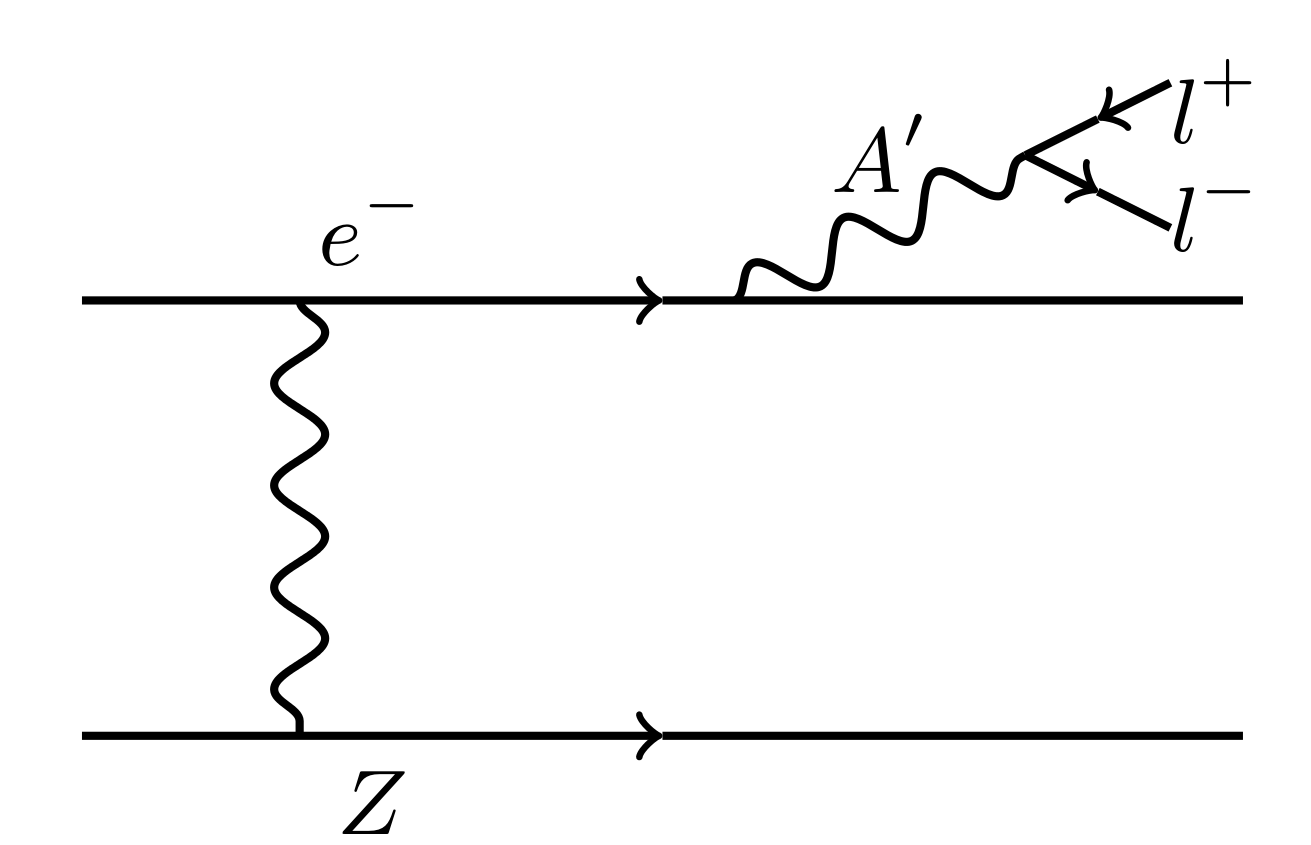
\includegraphics[width=0.5\textwidth]{images/aprime_brem.png}
    \label{fig:ap_production}
\end{figure}  
%%%%%%%%%%%%%%
%%%%%%%%%%%%%%
\cite{Bjorken2009, Tsai1986} where the process is viewed as the scattering of
photons sourced by the target nuclei by the incident electron in the rest frame
of the electron.  Therefore, the energy-angle distribution can be obtained from
the Compton-like process as
\begin{equation}
    \begin{split}
        \left[ \frac{d\sigma(e(p) + Z(P_i) \rightarrow e(p') + A'(k) + Z(P_f))}{dx d\cos\theta_{A'}} \right]_{W.W.} = \\
        \left( \frac{\alpha \chi}{\pi} \right) \left(\frac{E_0 x \sqrt{ 1 - m_{A'}^2/E_0^2}}{(1 - x)} \right) 
        \frac{d\sigma(e(p)\gamma(q) \rightarrow e(p') A'(k))}{d(p \cdot k)} |_{t = t_{min}} = \\
    \frac{8 \alpha^{3} \epsilon^{2} E_{0}^2 x \sqrt{1-m_{A'}^{2}/E_{0}^{2}}}{U^{2}} \chi
    \left [ \left (1 - x + \frac{x^{2}}{2} \right )  - \frac{(1-x)^{2} m_{A'}^{2}}{U^{2}}
    \left(m_{A'}^{2} - \frac{Ux}{1-x} \right) \right]
    \end{split}
    \label{eqn:ap_diff_cross}
\end{equation}
where $\alpha \sim 1/137$ is the fine structure constant, $\theta_{A}$ is the
opening angle of the $A'$ relative to the incident electron in the lab frame, 
$x = E_{A'}/E_{0}$ is the fraction of the incident electron energy carried by
the $A'$ and $m_A'$ is the mass of the heavy photon. The function 
\begin{equation}
    U(x, \theta_{A'}) = E_{0}^{2}x\theta_{A'}^{2} 
    + m_{A'}^{2}\frac{1-x}{x} + m_{e}^2 x
\end{equation}
is related to the virtuality of the intermediate electron while the effective
photon flux is related to the electric form factor
\begin{equation}
    \chi = \int_{t_{min}}^{t_{max}} \left(G_{2,el}(t) + G_{2,in}(t) \right] \frac{t - t_{min}}{t^2} dt
\end{equation}

Assuming $m_{e} << m_{A'}$, 
and integrating \ref{eqn:ap_diff_cross} over all angles yields
\begin{equation}
    \label{eqn:ap_diff_cross_i}
    \frac{d\sigma}{dx} = \frac{8\alpha^{3}\epsilon^{2} \sqrt{1-m_{A'}^{2}/E_{0}^{2}}}
    {m_{A'}^{2}\frac{1-x}{x} + m_{e}^{2}x}\chi
    \left( 1 - x + \frac{x^{2}}{3}\right).
\end{equation}
Although \ref{eqn:ap_diff_cross_i} reduces to the cross-section of photon 
bremsstrahlung in the limit that $m_{A'} \rightarrow 0$, their production rate
and kinematics differ in several ways. Specifically, the production 
cross-section is suppressed by a factor of $\epsilon^{2}m_{e}^{2}/m_{A'}^{2}$.
Furthermore, the $A'$ is produced very forward and will take most of the 
incident beam energy. \textbf{Expand this a bit more ... Also talk about the
total rates.}

\section{Trident Backgrounds}

The primary background expected to dominate the final event sample of the HPS 
experiment is the QED Bethe-Heitler and radiative trident processes.  Diagrams
on these processes are shown on Fig. \ref{fig:tridents}. The heavy photon 
signal is expected to appear as a resonance above the trident invariant mass
distribution so an understanding of these backgrounds is highly desirable. 
\begin{figure}[t]
    \begin{subfigure}{.5\textwidth}
        \centering
        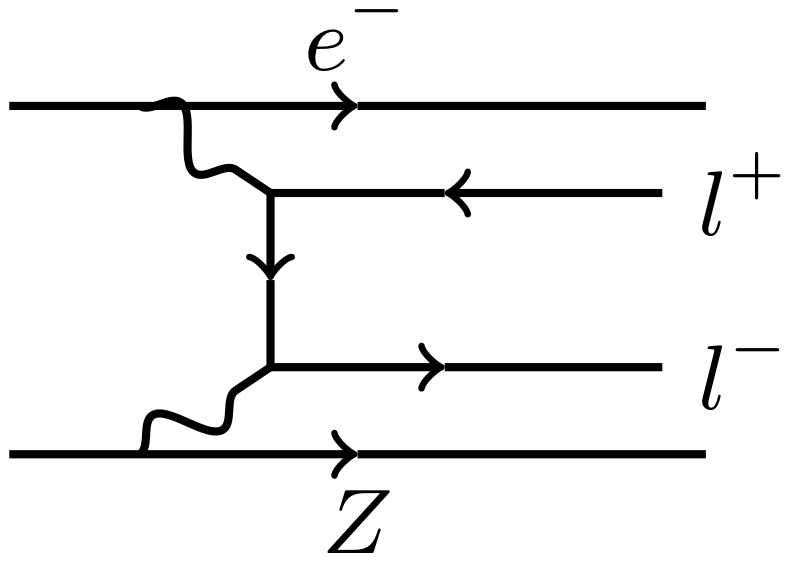
\includegraphics[width=0.8\textwidth]{images/bethe-heitler.png}
    \end{subfigure}
    \begin{subfigure}{.5\textwidth}
        \centering
        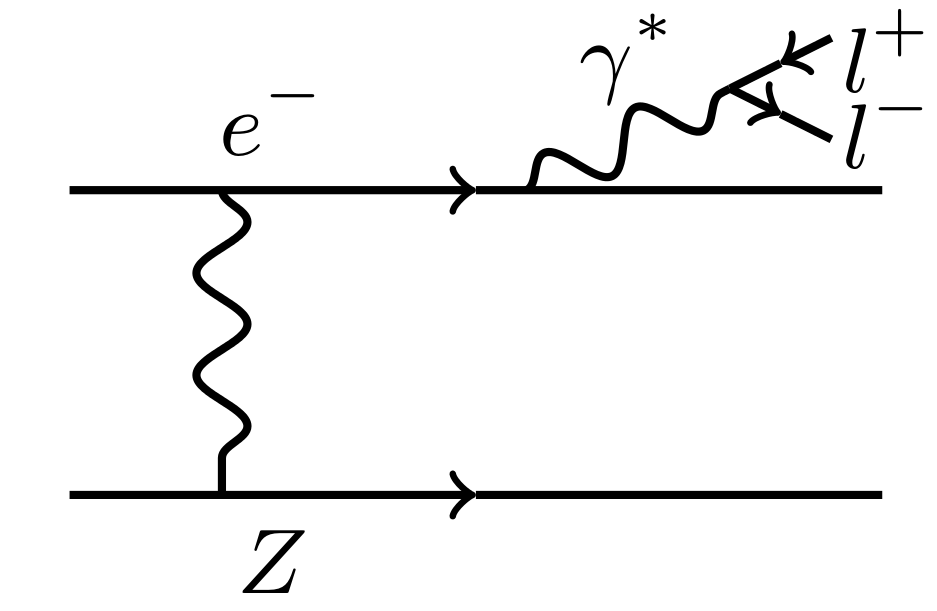
\includegraphics[width=0.8\textwidth]{images/radiative.png}
    \end{subfigure}
    \caption{Diagrams of the radiative and Bethe-Heitler trident reactions.}
    \label{fig:tridents}
\end{figure}  

The kinematics of radiatives are indistinguishable from $A'$ signal events 
within an invariant mass window, $\delta m$, near $m_{A'}$. Specifically, 
the $A'$ production cross-section is related to the production cross-section of 
radiatives as 
\begin{equation}
    \frac{d\sigma(e^-Z\rightarrow e-Z(A'\rightarrow l^+l^-))}
    {d\sigma(e^-Z\rightarrow e-Z(\gamma^*\rightarrow l^+l^-))}
    = \frac{3\pi\epsilon^{2}}{2 N_{eff} \alpha} \frac{m_{A'}}{\delta m}.
\end{equation}
Therefore, radiatives can be used to analyze both the rate of the $A'$ signal 
production and the sensitivity of an experiment to $A'$ signals.

Although the rate of the Bethe-Heitler process dominates among the two 
processes, its different kinematics can be used to reduce them in the final 
event sample.  Specifically, the $A'$ decay products are highly boosted while 
the recoiling electron is soft and scatters at large angles.  In contrast, 
at higher energies, the Bethe-Heitler process is not enhance.  Furthermore,
only one of the leptons in the pair will be highly boosted, while the other
will be much softer.  The recoiling electron will be produced much more forward.
These kinematic differences are illustrated in Fig. \ref{fig:ap_v_bethe}.
\begin{figure}[t]
    \centering
    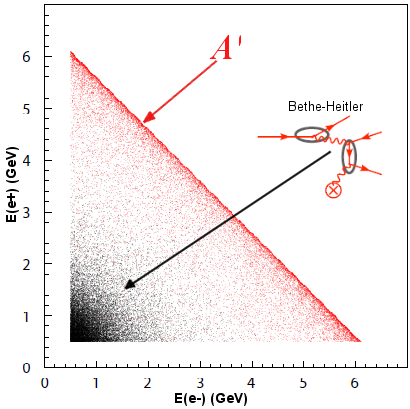
\includegraphics[width=0.5\textwidth]{images/bh_energy_cut.png}
    \caption{The distribution of the energy of the positron versus the electron
    for Bethe-Heitler (black) and $A'$ (red) event.}
    \label{fig:ap_v_bethe}
\end{figure}


